\chapter{Mécanismes de sécurité et mise en production}

\section{Protections générales}
\subsection{Durée de la session}
Par défaut, les sessions ont une durée de vie d'une heure sans activité. Elles sont supprimées automatiquement, sans tenir compte le cas échéant du cookie de session. Ce dernier est transmis en \textit{http\_only} et en mode \textit{secure}.

Si la session dure plus d'une heure\footnote{la durée par défaut de la session}, l'identifiant de session est régénéré.

\subsection{Protection contre le changement d'adresse IP}

Si l'adresse IP du client change pendant la session, celle-ci est fermée. L'adresse IP récupérée tient compte, le cas échéant, d'un passage par un serveur \textit{Reverse-Proxy}.

\section{Intégrer le transcodage des clés}

Dans certains cas de figure, l'utilisateur ne peut traiter que certains enregistrements d'une table. Le framework dispose d'une classe qui permet de transcoder les clés, pour éviter que l'on puisse modifier indûment une clé.

la classe \textit{TranslateId} (fichier \textit{framework/translateId/translateId.class.php}) permet de gérer le transcodage des clés.

Cette classe doit être instanciée en variable de session.

\subsection{Charger le fichier de classe avant le démarrage de la session}

Dans \textit{modules/beforesession.inc.php}, rajoutez la ligne suivante :
\begin{lstlisting}
require_once 'framework/translateId.translateId.class.php';
\end{lstlisting}

\subsection{Instancier la classe}
Voici un exemple d'instanciation :
\begin{lstlisting}
if (!isset($_SESSION["ti_table"]) 
	$_SESSION["ti_table"] = new TranslateId("id");
\end{lstlisting}

\textit{id} correspond au nom de la colonne à transcoder.



\chapter{Mise en production}

\section{Configuration et installation générale}

\subsection{Configuration du serveur web}

\subsection{Nettoyage de l'application et contrôles à réaliser}

\subsection{Installation de la base de données des droits}

\subsection{Nettoyage des comptes par défaut}

\section{Travailler avec plusieurs applications différentes à partir du même code}\label{dnsmultiple}

Dans certains cas, l'application réalisée doit permettre de travailler avec des bases de données différentes selon le contexte, pour éviter de mélanger les informations. La première solution consiste à créer autant de copies que nécessaire du logiciel.

La seconde consiste à n'utiliser qu'un seul code, mais en paramétrant les informations spécifiques à chaque base de données.

Voici le principe général (\textit{cf.} schéma \ref{dnsmultipleschema})  :
\begin{figure}[th]
\label{dnsmultipleschema}
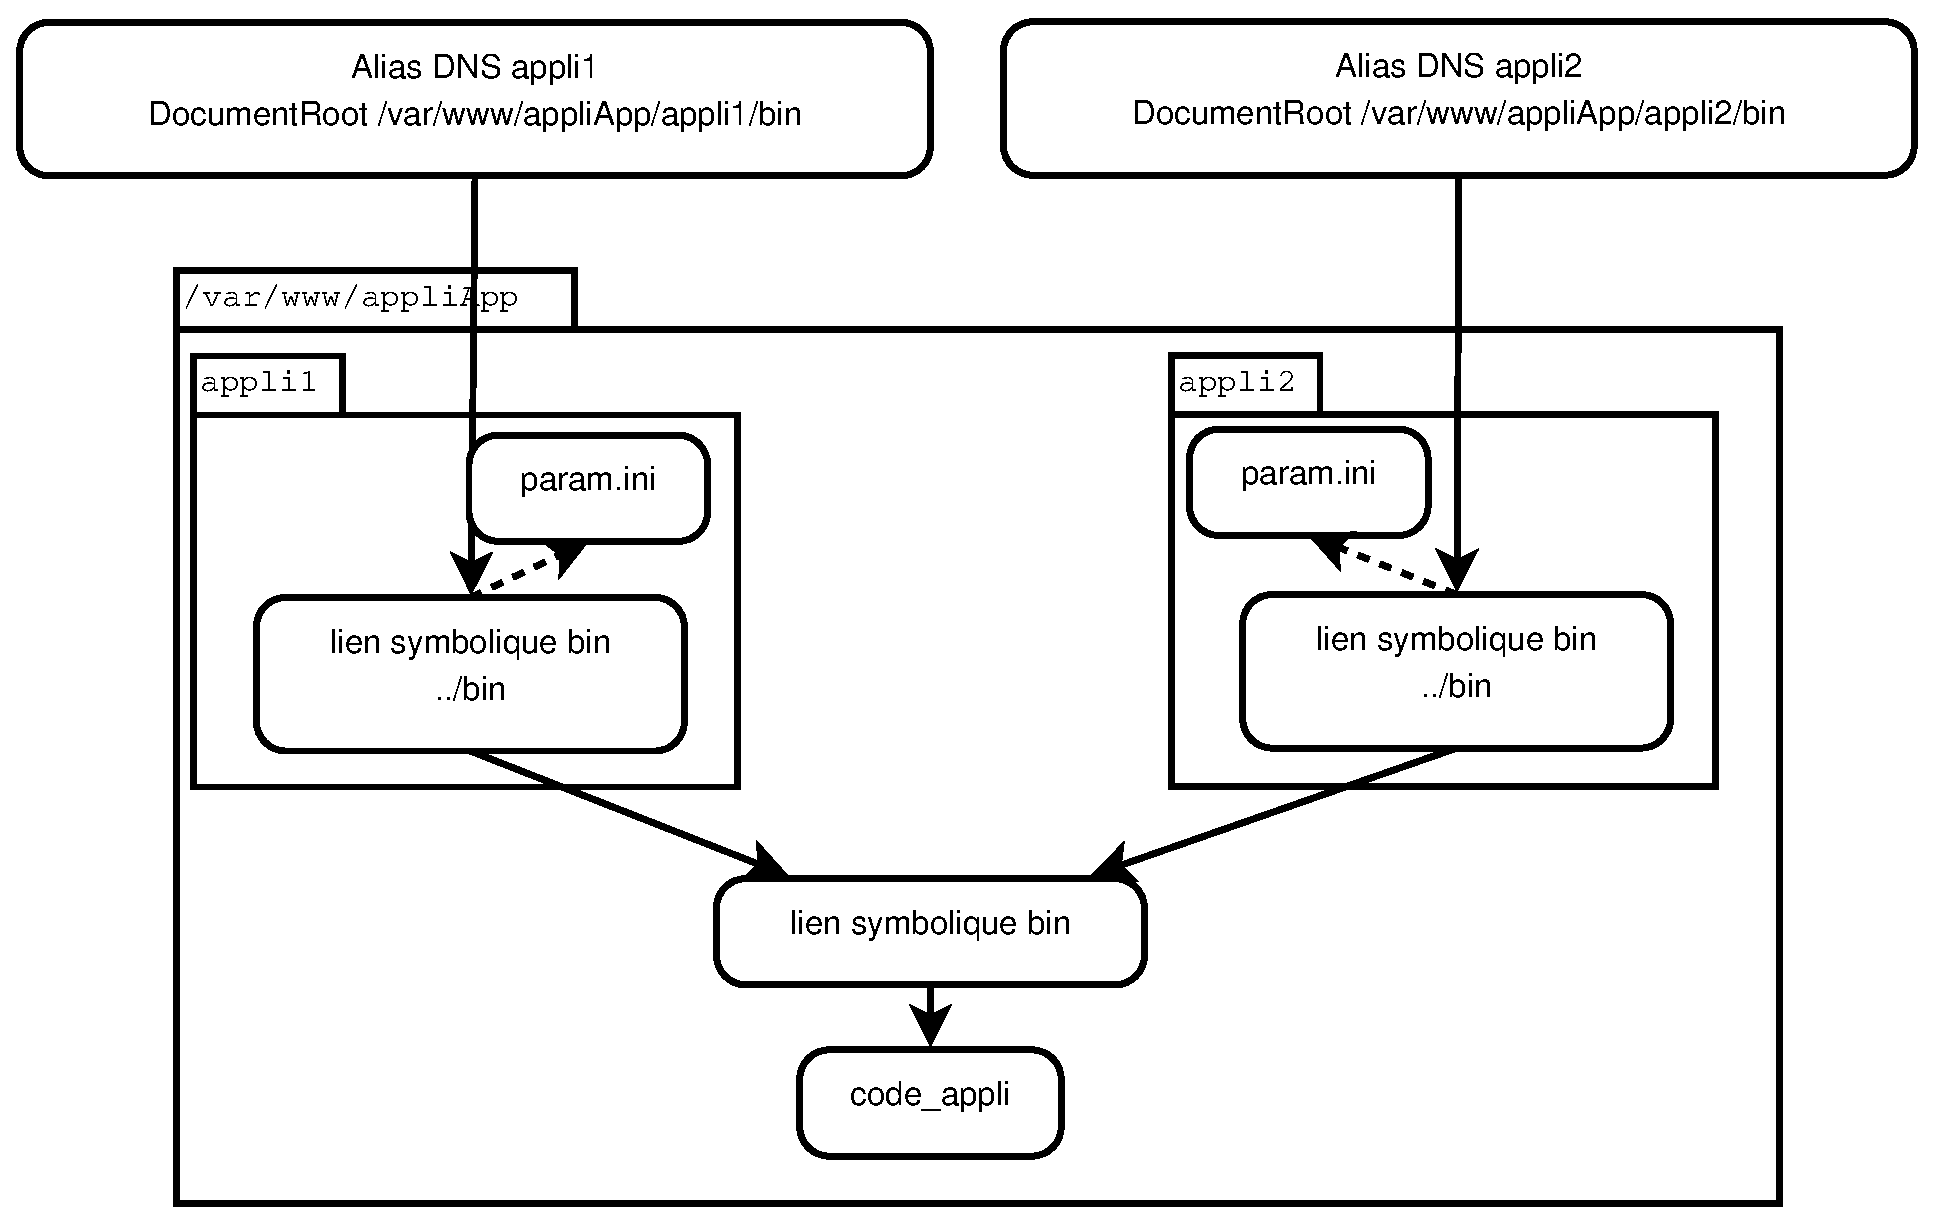
\includegraphics[width=\linewidth]{dessin/dnsmultiple}
\caption{Schéma général d'implémentation pour utiliser le même code avec des noms d'application et des jeux de données différents}
\end{figure}

Dans le paramétrage de l'alias DNS (en principe, dans \textbf{/etc/apache2/sites-available}), l'application pointe vers le dossier \textbf{/var/www/appliApp/appli1/bin}. 
\textit{/var/www} correspond à la racine du site web, \textit{appliApp} au dossier racine de l'application, \textit{appli1} au dossier spécifique de l'alias DNS.

Ce dossier \textit{appli1} ne contient que deux fichiers : \textbf{param.ini}, qui contient les paramètres spécifiques, et \textbf{bin}, qui est un lien symbolique vers le dossier \textbf{../bin}. 

Le dossier \textit{../bin} (donc, dans \textit{/var/www/appliApp}) est lui aussi un alias qui pointe vers le code réel de l'application, ici \textbf{code\_appli}.

Le fichier \textbf{param.inc.php} décrit l'entrée suivante :
\begin{lstlisting}
$paramIniFile = "../param.ini";
\end{lstlisting}

Le fichier \textbf{param.ini} sera cherché dans le dossier parent du code de l'application, c'est à dire soit dans \textit{appli1}, soit dans \textit{appli2} dans cet exemple.

Il suffit qu'il contienne les paramètres adéquats pour rendre l'application utilisable dans des contextes différents à partir du même code initial.